\chapter{Solitary wave run-up (tests\_channel)}

\section{Purpose}
This project aims to simulate the solitary wave run-up tests described in
Synolakis in 1986 \cite{Synolakis1986} and in 1987 \cite{Synolakis1987} using a range
of numerical models. Those tests were performed in a wave flume with a model
beach of slope 1:19.85. Solitary waves were generated at a distance of 14.68~m
from the toe of the model beach.

A similarly sized domain will be created using a numerical model. Solitary
waves be generated at the boundary, allowed to propagate through the domain and
run-up will be extracted.  The extracted values of run-up can then be compared
to the physical modelling data and assessment made of the model accuracy.

\section{Description}

The configuration is a 50~m long and 1~m large channel.

\subsection{Geometry and mesh}

Figure~\ref{fig:tests:geometry} shows the geometry of the study.

\begin{figure}[H]
\centering
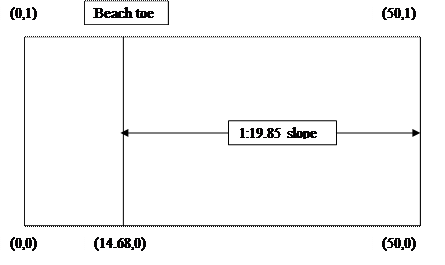
\includegraphics[width=.6\textwidth]{img/geometry.png}
\caption{Geometry of the study.}
\label{fig:tests:geometry}
\end{figure}

The mesh is made of 20,000 regular triangles and 11,011 nodes
(see Figure~\ref{fig:tests:mesh}).

\begin{figure}[H]
\centering
\includegraphicsmaybe{[width=.6\textwidth]}{../img/Mesh.png}
\caption{Mesh of the study.}
\label{fig:tests:mesh}
\end{figure}

Figure~\ref{fig:tests:bathy} shows the bathymetry of the study.

\begin{figure}[H]
\centering
\includegraphicsmaybe{[width=.6\textwidth]}{../img/Bathy.png}
\caption{Bathymetry of the study.}
\label{fig:tests:bathy}
\end{figure}

\subsection{Boundaries}

Solid Wall all around.

Solitary wave :

$\eta(0,t) = H \rm{sec } h^{2}(\gamma c(t-T_{1}))$ with $\gamma=(\frac{3H}{4d^{3}})$ and
$c=\sqrt{gd}(1+\frac{H}{2d}-\frac{3H^{2}}{20d^{2}})$

Figure~\ref{fig:tests:params} gives a list of parameters of the simulations.

\subsection{Numerical parameters}
\begin{figure}
\centering
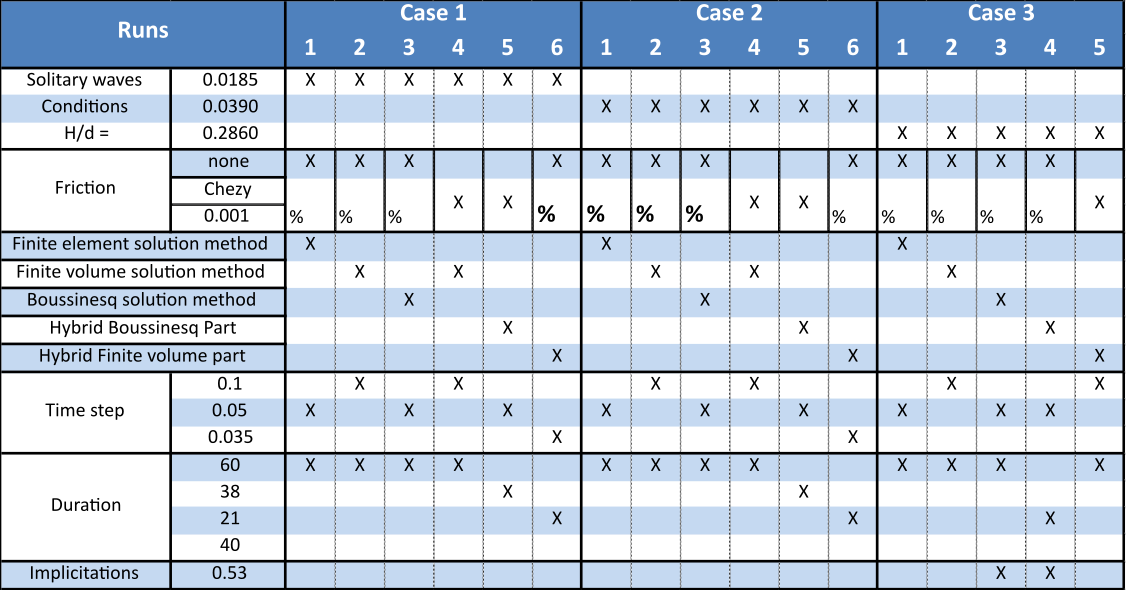
\includegraphics[width=.6\textwidth]{img/run_param.png}
\caption{List of parameters.}
\label{fig:tests:params}
\end{figure}

\section{Results}

The results obtained with \telemac{2D} simulation and Synolakis for cases 1, 2
and 3 are presented in Table 1. The \telemac{2D} wave run up results versus the
physical model results are presented in the scatter plotwith the empirical
relationships obtained by Synolakis displayed for reference.

%\section{Results}
\subsection{Case 1}

It can be seen, from Table \ref{tab:tests:runup} and Figure 3 that the maximum
run-up values are in reasonable agreement with the values obtained by Synolakis.
The finite volume (with friction) and hybrid solution methods are in excellent
agreement with the experimental value.

\begin{table}[H]
  \begin{center}
  \begin{tabular*}{.9\textwidth}{|*{7}{c|}}
\hline
  & Case          & Wave Run-up (R/d) & & & & \\
\hline
  & Synolakis    & FE    & FV    & Boussinesq & FV with $C_f$ = 0.001 & Hybrid \\
\hline
1 & 0.076, 0.078 & 0.068 & 0.084 & 0.068      & 0.077 & 0.076 \\
\hline
2 & 0.162        & 0.103 & 0.199 & 0.107      & 0.155 & 0.156 \\
\hline
3 & 0.513        & 0.148 & 0.497 & 0.135      & -     & 0.535 \\
\hline
  \end{tabular*}
  \end{center}
  \caption{Maximum run-up (experiments and simulations.}
  \label{tab:tests:runup}
\end{table}

Figure~\ref{fig:tests:res} shows the comparison with the benchmark data.
\begin{figure}
\centering
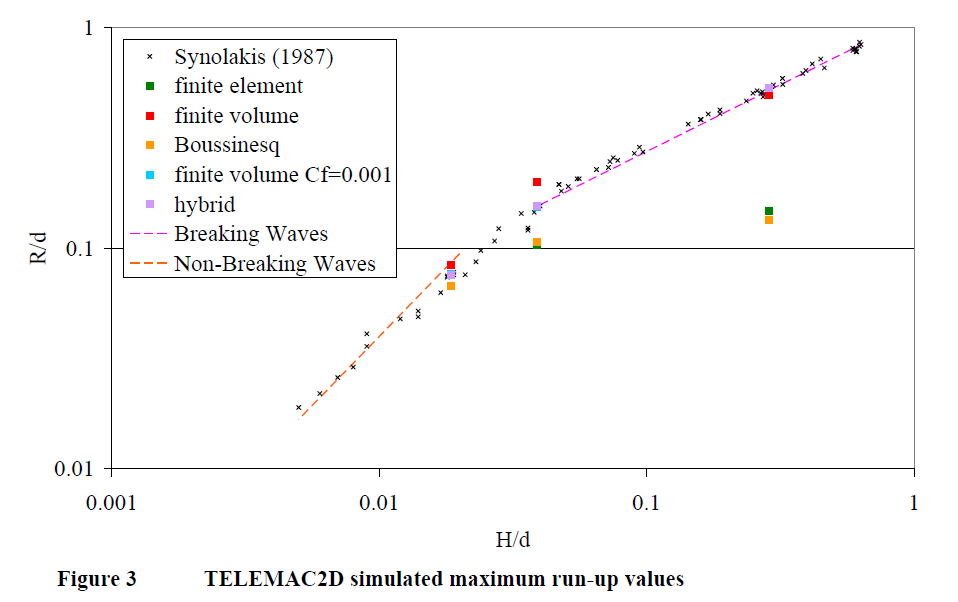
\includegraphics[width=.8\textwidth]{img/fig3.png}
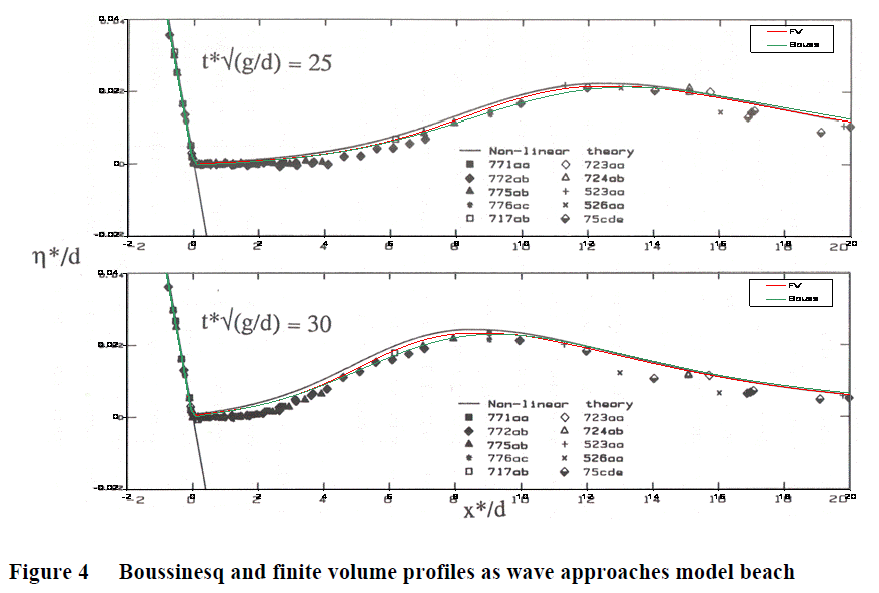
\includegraphics[width=.8\textwidth]{img/fig4.png}
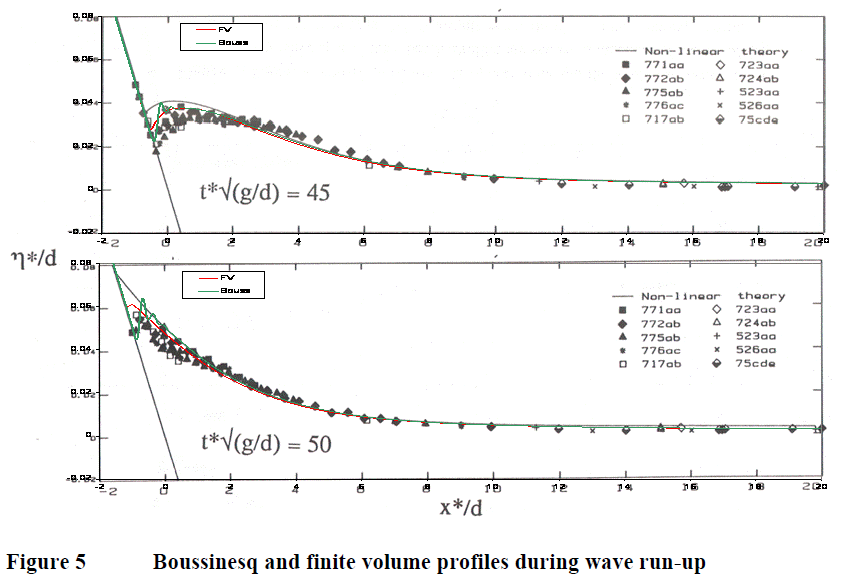
\includegraphics[width=.8\textwidth]{img/fig5.png}
\caption{Comparison with the benchmark data.}
\label{fig:tests:res}
\end{figure}

\subsection{Case 2}

The results in this case follow a broadly similar pattern to that obtained for
Case 1, presented above.  Again a hybrid solution method is essential to model
accurately all phases of the wave profile development.

\subsection{Case 3}

Figure~\ref{fig:tests:case3} shows the results for the case 3.
\begin{figure}[H]
\centering
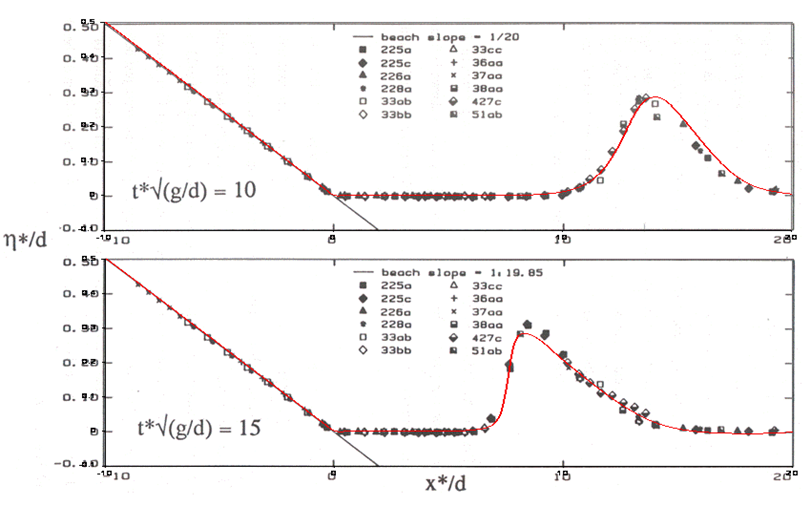
\includegraphics[width=.6\textwidth]{img/case3.png}
\caption{Velocity vectors over the free surface.}
\label{fig:tests:case3}
\end{figure}


Figure~\ref{fig:tests:chezy} shows the results for the case 3.
\begin{figure}[H]
\centering
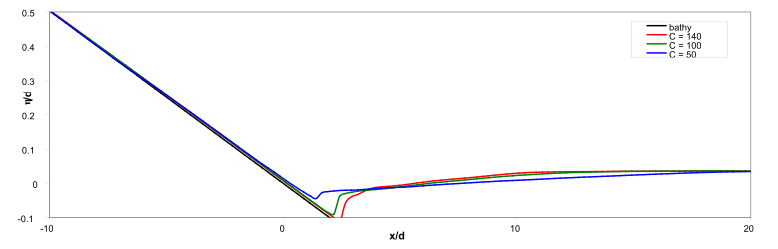
\includegraphics[width=.6\textwidth]{img/chezy1.png}
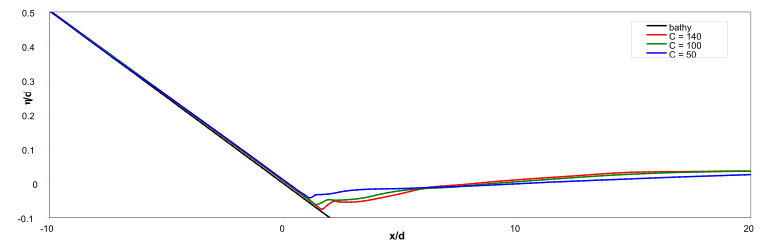
\includegraphics[width=.6\textwidth]{img/chezy2.png}
\caption{Chézy friction factors of 140, 100 and 50 (which correspond to Cf values of.}
\label{fig:tests:chezy}
\end{figure}

Chézy friction factors of 140, 100 and 50~m$^{1/2}$/s (which correspond to $C_f$ values of
0.001, 0.002 and 0.008 respectively).

The inadequacy of the finite element and Boussinesq solution methods for this
case is clear from inspection of Table \ref{tab:tests:runup} and Figure 3.
The finite volume
method appears to perform better (from consideration of the run-up value alone)
but, on closer inspection of the wave propagation, it can be seen that the wave
shape was not adequately maintained, deforming significantly from the input
profile before reaching the beach slope. All three solving methods result in a
dramatic reduction in the peak wave height before the wave reaches the beach
slope.

The hybrid method performed better, with a good representation of the wave
approach and run-up.  The wave run-down was less well modelled, with the
thickness of the fluid layer being badly reproduced. It was theorised that the
friction factor used is not large enough and so a sensitivity study was
performed using Chézy friction factors. It was found however that increasing
the friction factor had very little impact on the thickness of the fluid layer
in the wave run-down phase, and reduced the magnitude of the hydraulic jump
attained as the wave ran down the slope.

\section{Conclusion}

Only hybrid method can capture the development of the wave on the flat bed and
model beach and match the maximum run-up:
\begin{itemize}
\item Point of wave breaking needs to be decided a posteriori,
\item Tuning of the numerical Boussinesq solution method is required to propagate large waves,
\item Friction is crucial to limit run-up.
\end{itemize}
